\section{Cahier des charges}
    Le but premier de ce projet est de réaliser un outil permettant à un utilisateur (potentiellement) novice d'effectuer une analyse sur la sécurité de son système, quelle qu'en soit sa nature. Cette analyse devra ensuite lui permettre de mettre en place les défenses les plus adaptées et les plus "rentables", jusqu'à obtention d'un système dont la sécurité le satisfait pleinement.
    
    L'analyse reposera grandement sur l'utilisation d'arbres d'attaque--défense, mais aussi sur une expertise (extérieure ou non) pour pouvoir valuer les feuilles des arbres\footnote{C'est d'ailleurs à cet endroit qu'un utilisateur novice rencontrera le plus de difficulté.}.
    
    L'outil prendra la forme d'une suite logicielle, dont les différents composants réaliseront chacun une fonctionnalité précise et devront interagir ensemble, et listé ci dessous:
    \begin{itemize}
    	\item Une bibliothèque de modèles d'attaques existantes (détaillé dans la sous-section \ref{subsec:biblio_atk}).
        \item Un guide (plus ou moins interactif) pour partir de zéro, même novice (sous-section \ref{subsec:guide_inter}).
        \item Un éditeur d'arbres (sous-section \ref{subsec:edit_arbre}).
    \end{itemize}

    \subsection{Spécifications générales}
        \label{subsec:spec_gen}
        L'analyse du client sera sauvegardée sous forme de projet. Lorsque l'utilisateur voudra créer une nouvelle analyse, il devra créer un nouveau projet, et répondre à une série de questions, comme le type du système, l'attaquant imaginé, et bien d'autre.
        
        Ces informations permettront de présélectionner des modèles plus pertinents au cas de l'utilisateur, et pourront par exemple nous servir à générer un arbre de base. L'utilisateur pourrait alors l'éditer pour obtenir un arbre d'attaque correspondant à sa situation.
    
    \subsection{Architecture}
        Nous avons décidé de partir sur une architecture modèlaire, où une application mère, qui servira de chef d'orchestre, sera chargé de lancer les différents composants, chacun spécifique à une tache en particulier. % Trop long, reformuler.
        Un ébauche de l'architecture envisagée est disponible figure \ref{fig:archi}.

        \begin{figure}
            \begin{center}
                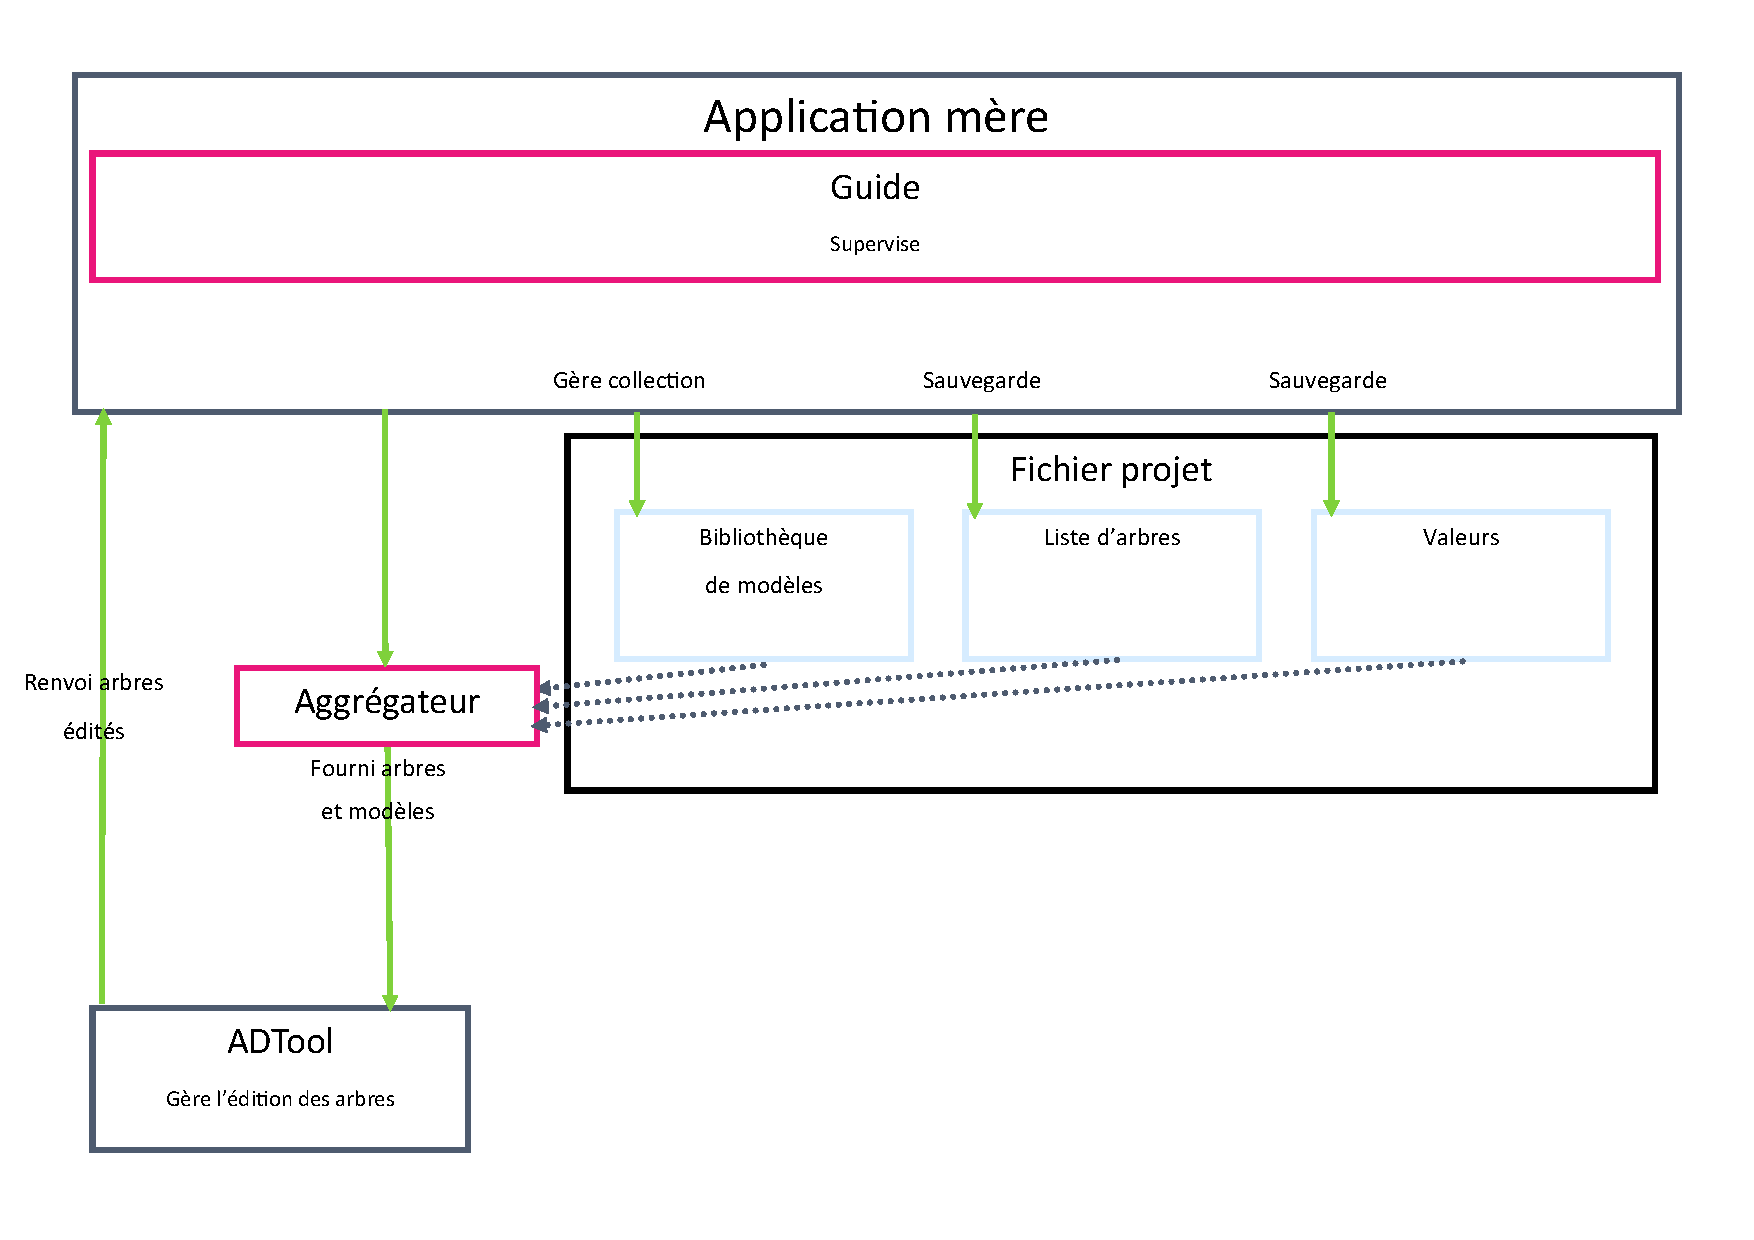
\includegraphics[width=1\textwidth]{figure/archi.pdf}
            \end{center}
            \caption{Différents composants interviendront pour éditer le fichier projet.}
            \label{fig:archi}
        \end{figure}

        % Reformuler ce merdier
        La spécialisation des composants nous permettra d'optenir une architecture logicielle plus propre, qui facilitera le développement: chaque partie sera indépendante des autres, et les choix techniques de l'une ne limiteront pas une autre.

        Avec ce choix d'architecture modulaire, nous réaliserons donc plusieurs outils spécialisés, mais qui le feront bien, plutôt que faire une seule grosse application qui fera tout de manière médiocre et dont l'architecture rendra toute modification très difficile.
        
        De plus, cette architecture peut potentiellement nous permettre de réutiliser certains outils dans d'autres contextes, ou encore de remplacer un des logiciel par un autre sans trop de difficulté. 
    
    \subsection{Bibliothèque d'attaques}  
        \label{subsec:biblio_atk}
        La bibliothèque d'attaques servirait à décrire des cas très généraux, que l'utilisateur pourrait détailler en fonction de sa situation. 
        
        Afin de garder les choses lisibles et ne pas surcharger les autres projets, chaque projet stockera sa propre bibliothèque. De plus, cela rendra la copie de projets entre différents ordinateurs plus aisée.
        
        La bibliothèque d'attaques du projet sera préchargée de diverses attaques en fonction des réponses de l'utilisateur lors de la création du projet, et pourra par la suite être complétée (ou épurée, c'est tout comme) en ajoutant des modèles de base (stockés par notre application) ou venants de l'internet sauvage.
        
        Dans notre exemple (la STAR), nous pourrons fournir des arbres d'attaque de réseaux de transport communs à toutes les villes de France, que nous pourront ensuite détailler pour la ville de Rennes.
      
    \subsection{Guide interactif}
        \label{subsec:guide_inter}
    	Le guide doit être capable d'expliquer à l'utilisateur comment faire son analyse. 
        
        Il pourra par exemple poser une série de questions à l'utilisateur, afin de générer un arbre dit "de base" sur lequel l'utilisateur pourra commencer son analyse.
        
        Chaque notion devra être expliquée de manière claire et concise.
        
        Découper l'analyse en différentes étapes. Une fois que l'utilisateur aura complété une étape, il faudra lui expliquer la suite.
        
        Nous pensions faire référence au célèbre trombone magique de Microsoft Office, mais, pour des raisons de droit, nous utiliseront à la place une agrafeuse.
        
    \subsection{\'Editeur d'arbres}
        \label{subsec:edit_arbre}
        Pour l'édition des arbres, nous utiliserons un outil préexistant, à savoir AD Tool\cite{adtool_paper}.  
        
        Toutefois, quelques modifications seront nécessaire, afin non seulement de rendre l'édition des arbres plus souple, mais aussi et surtout pour pouvoir plus facilement importer et exporter des arbres générés
        
        L'objectif en effet serait de faire générer un arbre par notre application mère à partir de différents modèles, pour ensuite demander à l'utilisateur de réaliser les finitions.
    
	\subsection{Multiplateforme}
        Bien que nous allons nous concentrer sur une seule plateforme d'utilisateur (à savoir, Microsoft WINDOZE), nous utiliseront des langages et librairies qui permettront facilement de rendre notre programme multiplateforme par la suite, si jamais on s’ennuie entre la pause café et la pause midi.

    \subsection{License}
    	ADTool: GPL3
        
        Nous souhaitons garder un logiciel open-source, parce que nous avons l'esprit du partage et souhaitons à l'humanité d'avoir un futur rose et plein d'arcs en ciel.
        
        En revanche, des méchants libristes ont mis au point un virus contaminant les applications libres, ce qui fait qu'on risque de devoir utiliser la GPL, même si on a pas vraiment vraiment envie.